The Large Hadron Collider (LHC)~\cite{LHC} is a two ring superconducting hadron
accelerator and collider located at the European Organization for Nuclear
Research (CERN).

The performance of a collider is evaluated in terms of its available
\emph{center of mass energy}, $\sqrt{s}$ and the \emph{instantaneous luminosity}
$\lumi$. The former defines the accessible phase space (the momenta) for the
production of final state particles. The latter is defined as the interaction
rate per unit cross section of the colliding beams (collisions / (cm$^2$
s)).

The LHC is designed to operate at $\sqrt{s} = 14$~TeV in the center of mass
although it started off at 7~TeV in 2010 and 2011, 8~TeV in 2012 and 13~TeV in
2015 after the long shutdown between 2013 and 2014.

There are six experiments at LHC: ATLAS~\cite{ATLASPaper},
CMS~\cite{1748-0221-3-08-S08004}, ALICE, LHCb, LHCf and TOTEM. ATLAS and CMS aim
to a peak luminosity of $L = 10^{34}$~cm$^{-2}$ s$^{-1}$, this requirement
exclude the use of anti-proton beams and therefore the LHC is designed to be a
proton-proton ($pp$) collider. The protons are obtained by ionization of
hydrogen atoms and organized in bunches, accelerated by LINAC2 to an energy of
50~MeV and subsequently injected in the Proton Synchrotron Booster (PSB). Here
they are further accelerated to an energy of 1.4~GeV and fed to the Proton
Synchrotron (PS) where they reach the energy of 25~GeV to be then passed to the
Super Proton Synchrotron which accelerate them to an energy of 450~GeV. They are
finally injected in the LHC in opposite direction where they reach the nominal
energy. There are four interaction points where the four main experiments
(ATLAS, CMS, ALICE, LHCb) are located, at these locations, every 25~$\mu$s, the
bunches cross and interact with each other (\emph{bunch crossing}). A schematic
view of the injection chain is depicted in Figure~\ref{fig:lhc_inj_chain}.

The instantaneous luminosity depends on the beam parameters and is given by:
\begin{equation}
  \label{eq:54}
  \lumi = \frac{N^2_b n_b f_{rev} \gamma}{4 \pi \epsilon_n \beta^*} F
\end{equation}
where $N_b$ is the number of particles per bunch, $n_b$ is the number of bunches
per beam, $f_{rev}$ is the revolution frequency, $\gamma$ is the relativistic
gamma factor, $\epsilon_n$ the normalized transverse beam emittance, the beta
function is a measure of the transverse beam size and $\beta^*$ is the value of
the beta function at the interaction point and $F$ is the geometric reduction
factor due to the crossing angle of the beams at the interaction point
(IP)~\cite{LHC}. The integrated luminosity is given by:
\begin{equation}
  \label{eq:55}
  L = \int \lumi \ud t
\end{equation}
and the integral is carried over data taking periods of the detector. The
integrated luminosity can be related to the total number of events by:
\begin{equation}
  \label{eq:56}
  N_{events} = L \sigma_{events}
\end{equation}
where $N_{events}$ is the total number of events, $L$ is the integrated
luminosity and $\sigma_{events}$ is the cross section of the events in units of
barn (1~b = 10$^{-24}$~m$^2$). In 2015 ATLAS recorded an integrated luminosity
of 3.2~\ifb.

\begin{figure}[!h]
  \centering
    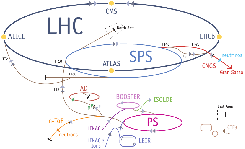
\includegraphics[width=.5\linewidth]{lhc_inj_chain}
    \caption{The LHC injection chain.}
    \label{fig:lhc_inj_chain}
\end{figure}
%%% Local Variables:
%%% mode: latex
%%% TeX-master: "../search_for_DM_LED_with_ATLAS"
%%% End:
